\section{Introducción}


En las últimas décadas la investigación en fuentes alternativas de energía ha recibido particular atención y ha pasado de tener un alto interés en los círculos académicos a convertirse en un punto prioritario en la agenda de gobiernos y organizaciones a nivel mundial.  La dependencia en combustibles fósiles y acuerdos internacionales como el protocolo de Kyoto han impulsado aún más el interés alrededor del tema.  En particular, la implementación de soluciones como páneles fotovoltáicos, parques eólicos y plantas de biomasa han atraido gran atención en especial en zonas con baja o nula cobertura.

En Colombia, según estudios del Ministerio de Minas y Energía, en el departamento de Nariño hay 15 municipios con cobertura eléctrica inferior al 80\% \cite{ministerio_de_minas_y_energia_plan_2008}. Como nueva estratégia para enfrentar esta problemática se ha propuesto el estudio y análisis de fuentes alternativas de energía en la zona. Uno de los principales objetivos es la medición y estimación de potenciales energéticos para identificar las zonas más viables en la región donde efectuar pruebas piloto y estudios de factibilidad. 

Sin embargo, uno de los principales retos para la ubicación de dichas zonas es la ausencia de bases de datos actualizadas así como series de tiempo históricas que apoyen el proceso de toma de decisiones.  Igualmente, restricciones de tiempo y costos impiden el despliegue de trabajo de campo para la recolección de información.  En el caso del análisis del potencial biomásico, estas restricciones se acentuan debido a la toma manual de muestras, extensión del área de estudio, análisis de laboratorio, dificultad del terreno e, incluso, presencia de grupos armados en la zona. 

En este sentido, diversas investigaciones han demostrado la utilidad del uso de imágenes satelitales para la generación de modelos que permitan calcular la cantidad de biomasa presente en un determinado lugar. Desde hace más de 30 años, se cuenta con acceso al repositorio de imágenes satelitales Landsat \cite{landsat} de manera libre y gratuita.  Bajo el debido tratamiento, estas imágenes pueden ser usadas para calcular valores nominales de biomasa a partir de modelos de regresión y trabajo de campo.  Sin embargo, dadas las dificultades para realizar dicho trabajo de campo, este estudio propone utilizar imágenes provistas por investigaciones anteriores.   \cite{baccini2008afirst} y \cite{baccini_estimated_2012} proporcionan bases de datos de los índices de biomasa a nivel pan-tropical entre los años 2000 y 2003.  Al igual que el conjunto de imágenes Landsat, las imágenes georreferenciadas para cada uno de los países analizados son de libre acceso y se encuentran disponibles en \cite{WHRC}.

Esta investigación presenta la metodología propuesta para la generación de un modelo de predicción de biomasa, basado en modelos de regresión e imágenes satelitales de libre acceso, y su extrapolación al resto del área de estudio.

El area de estudio de esta investigación fue el departamento de Nariño, el cual esta ubicado en el extremo Suroccidental de Colombia (en la frontera con Ecuador) con una extensión aproximada de 33.268 km, una población de 1,702 millones (según
el censo de 2013) y ubicada entre coordenadas 00° 31' 08'' y 02° 41' 08'' Norte y 76° 51' 19'' y 79° 01' 34'' Oeste (figura  \ref{fig:locationNarino}).

\begin{figure}
  \centering
  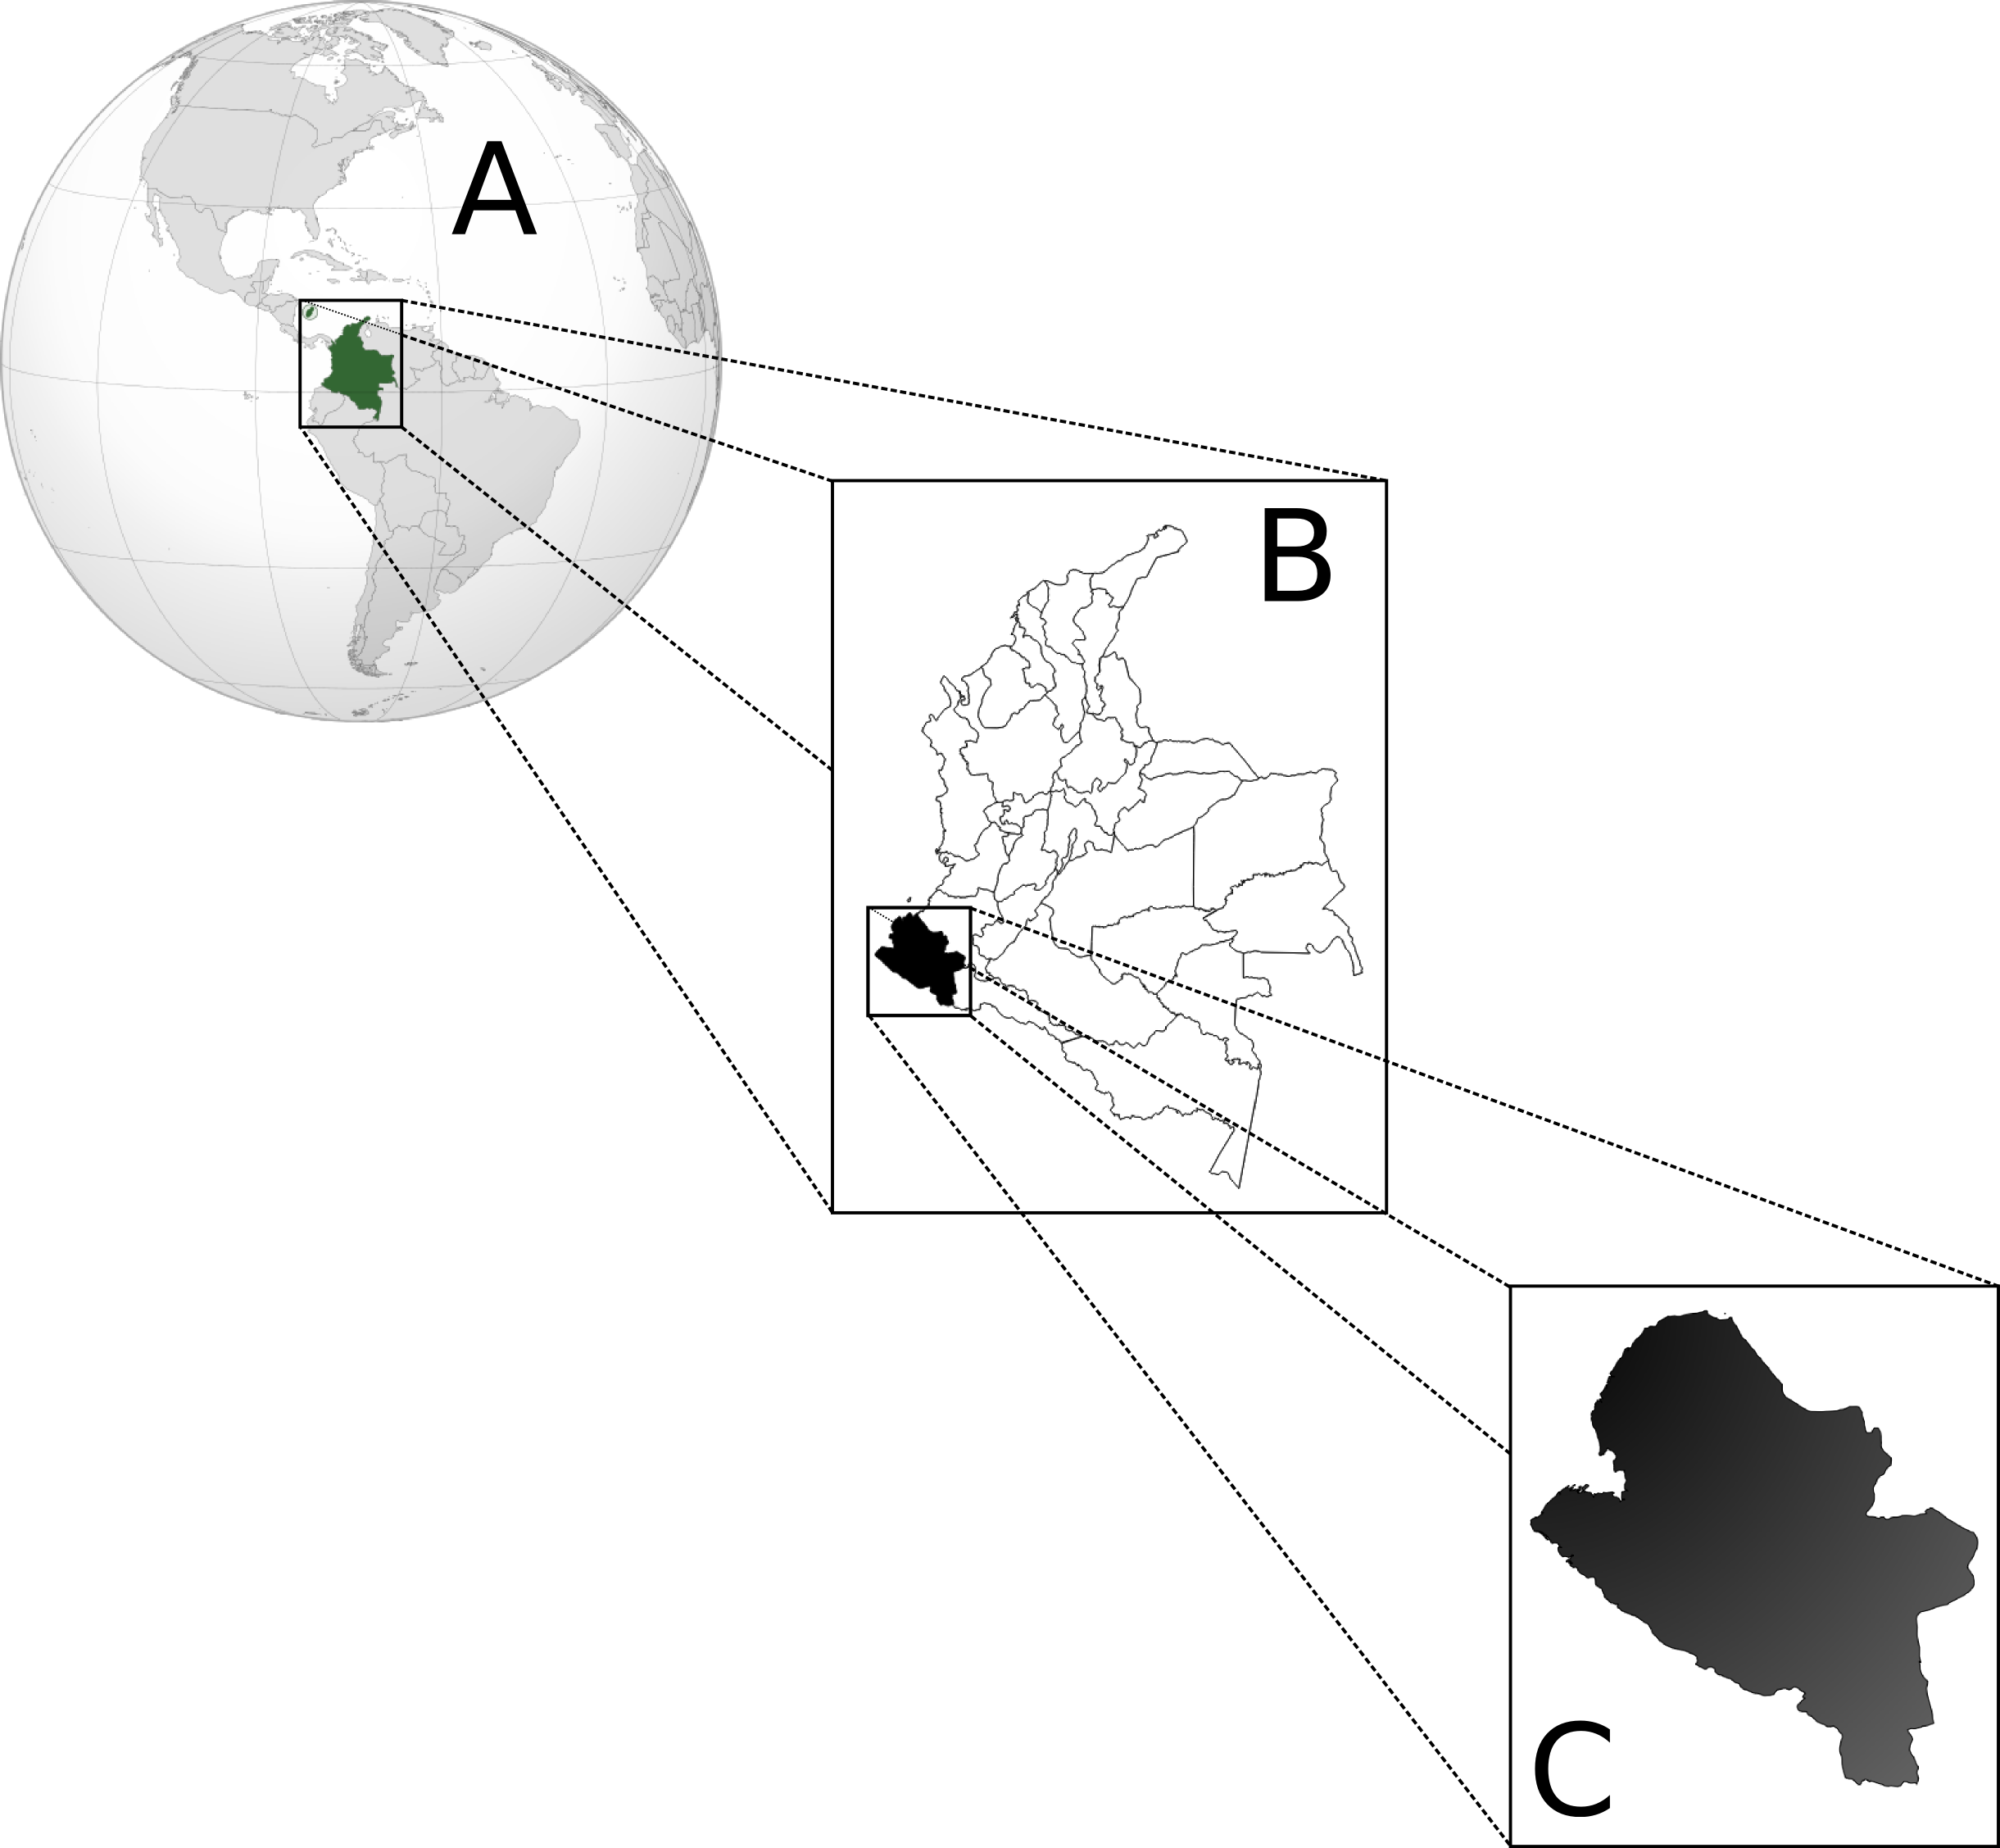
\includegraphics[width = 8cm]{locationNarino.png}
  \caption{Localización area de estudio}
  \label{fig:locationNarino}
\end{figure}